\begin{figure}
  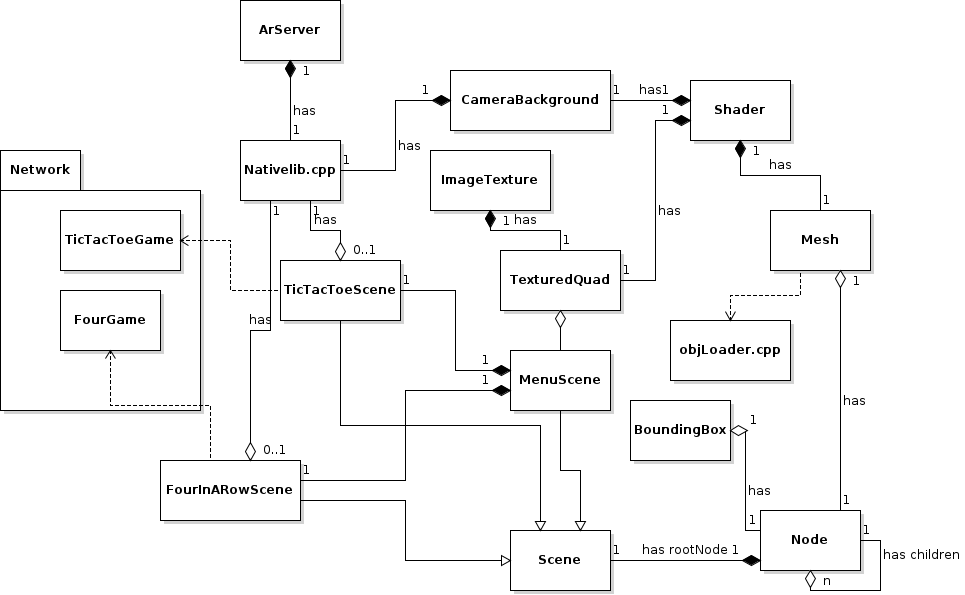
\includegraphics[width=\textwidth]{UML/ArCoreUML.png}
  \caption{Overview of the ArCore/GUI Part of the App}
\end{figure}
\subsection{Entwicklung eines Prototypen}
Am Anfang musste ich die Abhängigkeiten im Buildsystem auflösen, um
ArCore verlinken zu können. Zusätzlich musste ich mich mit dem grundlegenden Lebenszyklus von Apps
auseinander setzten und wegen Android NDK damit beschäftigen, wie man
Parameter von einer Java-Funktion an C übergibt.
Ich habe im nachhinen gemerkt, dass es die Möglichkeit gibt direkt in Android eine
´Native activity´\cite{android_native_activity} zu erstellen die nur C++ nutzt, aber alle OpenGL ES Code-samples von Google\cite{android_ndk_samples_2021},
sowie das AR-Core C Beispiel\cite{ar_core_sdk} nutzen Java mit eingehängten C++ und auch beim erstellen einer
´Native App´ in Android Studio, wird eine Java Activity mit gelinked C++-Code bereitgestellt.
\par
Daraufhin habe ich eine Dummy-
Implementation von ArCore geschrieben, um ArCore zum laufen zu bringen und besser zu verstehen.
Die Dokumentation von Google zu AR-Core war ein wenig kurz gefasst und ich musste dementsprechend immer wieder auf das Beispiel `\verb|hello_ar_c|`, um die Funktionsweise von ArCore zu verstehen.
Lange Zeit zeigte die Kamera kein Bild an, dabei stellte sich heraus das ArCore ein samplerExternalOES anstatt eines einfachen sampler2D benötigt.
\par
Danach merkte ich, dass der Android Emulator nur bedingt OpenGL ES 3.0 supportet\cite{android_emulator_gles3_issue},
deswegen musste ich den Code auf OpenGL ES 2.0 porten, was gerade wegen
Vertex-Array-Objects und eigene Sampler-Objects
umschreiben benötigt hat.
\par
Der Android Emulator hatte einen Bug und somit konnte ArCore App nicht
auf die virtuelle Kamera zugreifen. Das Problem bestand auch bei der Google Beispiel App
``\verb|hello_ar_c|``, aber auch in der Java Version.
\par
Da sich auch heraustellte, dass mein Smartphone ArCore nicht supportet, wurde ich darauf
aufmerksam, dass es eine Liste von supporten Geräten gibt. \cite{ar_core_supported_devices}
\par
Zu dem Zeitpunkt schlug unser Betreuer, Herr Uhlmann, vor auf OpenCV\cite{openCV} zu wechseln, um dementsprechend dem Problem
zu entgehen. Ich schaute mir OpenCV an, aber da die Entwicklung in OpenCV wohl einen sehr viel
größeren Arbeitsaufwand benötigt hätte, entschied ich mich ein ArCore supportetes Gerät zu kaufen.
\par
Auch unser Betreuer, war dementsprechend entgegen kommend und holte sich ein supportes Tablet.

\subsection{Funktionsweise von ArCore}
ArCore\cite{ar_core} ist eine Bibliothek von Google die unter Android ermöglicht AR Applikationen zu entwickeln.
ArCore analysiert dafür den Kamerastream und kann anhand dessen, die Umgebung erkennen.\\
ArCore bietet dafür folgendes:
\\ \\
arCamera: gibt einem Metainformationen über das Kamerabild,sowei eine Projektionsmatrix und Kameramatrix.
\\ \\
arPlane sind Oberflächen die von ArCore erkannt worden sind.(Wird automatisch generiert)
\\ \\
arPoint sind Punkte im reellen 3D Raum die erkannt worden sind.(Wird automatisch generiert)
\\ \\
arAnchor wird vom Entwickler erzeugt, arAnchor erwaret eine Bildposition(zumeist Touchposition), an dieser Bildposition versucht ArCore anhand von eigenen Daten (arPlane,arPoint), den Punkt auf dem geklickt wurde zu erzeugen. Wenn das geklappt hat, wird pro Kameraframe versucht diesen Anchor zu tracken und gibt für diesen Anchor eine Transformationmatrix zurück.


\subsection{Rendering}
\subsubsection{Erste Hilfsklassen}
Für das Rendering habe ich am Anfang ein paar Hilfsklassen gebaut:\\ \\
Shader in Shader.cpp für das lesen von Shadern aus Dateien, compilen und linken.\\ \\
objRenderer in objRenderer.cpp für das Rendern von obj-Files. Später wurde die
Funktionalität in die Mesh Klasse überführt.\\ \\
cameraBackground in cameraBackground.cpp, die das Kamerabild auf einen ScreenQuad sampelt.\\ \\
Aus dem \verb|hello_ar_c| von Google habe ich die objLoader.cpp entnommen, um obj-Dateien
laden zu können.
\subsubsection{Weitere Entwicklung}
Nachdem nun ArCore grundlegend lief habe ich einen Würfel erfolgreich geladen und rendern können.
Nachdem ich dann mit einem Klick auf dem Bildschirm einen
Anchor erzeugen lassen konnte und der Anchor richtig getracked wurde.
Habe ich dann ein simples Szenen System implementiert:
\\ \\
Mesh in Mesh.cpp, dieses lädt eine obj-Datei mithilfe von objLoader.cpp und ermöglicht das rendern dieses Meshes über draw().
\\ \\
Node in Node.cpp enthält
\begin{itemize}
  \item Mesh zum rendern
  \item ModelMatrix in Relation zur Elternnode
  \item Kinder, die auch Nodes sind
\end{itemize}
Scene in Scene.cpp, diese enthält die Root-Node.
Im Konstruktor der Scene werden die Nodes an die Root-Node angehängt oder an andere Nodes die schon angehängt wurden. Beim draw, wird das draw der Root-Node aufgerufen und jede Node ruft widderum
die draw Methode ihrer Childnodes auf und übergibt dabei die eigene Modelmatrix.
\\ \\
Damit wurde das Rendering sehr viel leichter und der Code sehr viel aufgeräumter.

\subsection{Probleme mit ArCore}
Das entwickeln mit ArCore verursachte mehrere Schwierigkeiten, dass größte Problem dabei war
die NDK(C) Version von ArCore. Dabei wurde die objektorientierte API in eine C-API
umgewandelt, was dazu führt, dass wenn in der Javaversion  ein Objekt ein anderes managed,
muss in C immer wieder das Objekt in Aufrufen mitgeschliffen werden.
\\
Hier ein Beispiel, um in der C API, die Modelmatrix von einem getrackten Punkt(anchor) zu bekommen:
\begin{verbatim}
ArPose *pose_;
ArPose_create(arSession, nullptr, &pose_);
ArAnchor_getPose(arSession, anchor, pose_);
ArPose_getMatrix(arSession, pose_, glm::value_ptr(modelMatrix));
ArPose_destroy(pose_);
\end{verbatim}
Siehe \cite{ar_anchor_c} für mehr Details.\\
Wie zu sehen, muss erst eine ArPose erstellt werden, die ArCore erzeugt, dann muss man an diese Pose, die Pose des Anchors binden und kann dann die ModelMatrix bekommen und am Ende muss die Pose wieder gelöscht werden. Dabei muss die arSession immer wieder übergeben werden.
Der gleiche Code in Java:
\begin{verbatim}
modelMatrix = anchor.getPose().toMatrix();
\end{verbatim}
Siehe \cite{ar_anchor_java} für mehr Details.\\
Somit hat es recht lange gedauert, bis ich einen guten Überblick über die C-API
hatte. Am Anfang hatte ich die API direkt in der Nativelib.cpp Datei, die die
Schnittstelle zwischen Java und C++ darstellt und habe diese später in arServer.cpp
migriert, was widerrum die Codekomplexität massiv senkte.

\subsection{Game}
Nachdem ich ArCore und ein gute Szenenabstraktion hatte, habe ich noch eine Hitbox detection geschrieben, diese basiert auf \cite{hitbox_detection}
die mir Herr Uhlmann gab.\\

Danach haben wir unsere beiden Entwicklungsbranches(Netzwerk, ArCore) gemerged, damit konnte ich
dann auf die GameStates zugreifen und dementsprechend für TicTacToe das Feld rendern.
Dabei sind keine größeren Probleme aufgetreten. \\

Da wir jetzt `Vier Gewinnt` implementieren sollten, habe ich die Scene zu einer vererbaren Klasse refactored (in TicTacToeScene.cpp) und daraufhin Vier gewinnt implementiert(FourInARowScene.cpp). \\

Zu guter Schluss habe ich ein Menü eingebaut, dass am Ende des Spiels angibt, ob man
verloren oder gewonnen hat und ein Button, um das Spiel neuzustarten.
Um den Text anzuzeigen habe ich einen TGA Loader geschrieben und musste
erfahren, dass vom Compiler nicht gewährleistet wird, dass structs tightly packed
sind, weshalb die Headerdaten der TGA nicht richtig ausgelesen wurden. Weswegen ich das Problem mehrere Stunden debuggen musste. Mit dem fertigen Menü, war dann auch die App fertig.
